\documentclass{article}
\usepackage[utf8]{inputenc}
\usepackage[ngerman]{babel}
\usepackage{graphicx}
\usepackage{amsmath}
\usepackage{booktabs}
\usepackage{textcomp}
\usepackage{multirow}
\usepackage{color}
\usepackage{listings}

\lstset{
	numbers=left,
	basicstyle=\small,
	tabsize=3,
	showspaces=false,
	showtabs=false,
	showstringspaces=false
}

\setcounter{tocdepth}{2}
\title{Aufgabenbl\"atter zum Praktikum: Anwendung und Programmierung im Grid}
\author{Ralph Krimmel \& Christian M\"uller}

\begin{document}
\maketitle{}
\vspace{2cm}
\begin{center}
	
\includegraphics[scale=0.4]{logo.png}
\end{center}
\newpage
\tableofcontents
\newpage
%\section{Aufgabenblatt 1}

\subsection{Aufgabe 1 - Grid Computing}

\subsubsection{Definiere Grid}
	\quotation{A computational grid is a hardware and software infrastructure that provides dependable, consistent, pervasive, and inexpensive access to high-end computational capabilities.}
	In einem Grid werden Ressourcen verwaltet und verteilt.
	Zusaetzliche Resourcen koennen bei Bedarf im Grid bereitgestellt werden.
	Die Ressourcen koenn dabei auf Verschiedene Weise gekoppelt werden:b
	Sequentiell, Verteilt oder Parallel
	Ein Grid wird von mehreren Personen oder Gruppen (VO) gleichzeitig verwendet.
	Sie geben ihre uebergeben ihre Aufgaben dem Grid,
	welches dann die bestmoegliche Art und Weise der Ausfuehrung ermittelt.
	
	Die Infrastruktur eines Grids besteht aus einzelnen Knoten,
	die die eingelntlichen Auftraege abarbeiten.
	Sie werden durch das Grid jedoch vor dem Nutzer versteckt und die Zuordnung der
	Aufgaben erfolgt durch spezielle Software (Grid Middleware).
	
\subsubsection{Vorteile von Grid-Technologie}
	\begin{itemize}
	  \item Gemeinsames Nutzen von teurer Hardware
	  \item Vereinfachung der Nutzung und erhoehte Portabilitaet
	\end{itemize}
	
\subsubsection{Anwendungen im Grid und deren Besonderheiten}
	Anwendungen im Grid muessen in der Lage sein,
	die ihnen gestellten Aufgaben in einzelne zu zerteilen.
	Diese Aufgaben koennen dann von den einzelnen Knoten verarbeitet werden.
	Dazu sind unter umstaenden bestimmte Anpassungen noetig.
	
\subsubsection{Definiere Grid-Middleware}
	Ein Grid-Middleware ist dafuer verantwortlich,
	dass sich ein Grid verhaelt wie ein einzelnes System.
	
	Sie vermittelt zwischen den laufenden Anwenungen und den lokalen
	Betriebssystemen der einzelnen Rechner/Knoten.
	
\subsection{Cluster Computing}
	\subsubsection{Skizziere eine Cluster Architektur und beschreibe die
	Wichtigsten Komponenten}
	\subsubsection{Welche Warteschlangenstrategien gibt es? Welche wuerdest du
	bevorzugen? Begruende!}
	
\subsection{Parallelisierung}
%\newpage
%\section{Aufgabenblatt 3}

\subsection{Torque Portable Batch System}
\subsubsection{Beschreibe die PBS Befehle}

\begin{description}
	\item[\texttt{qsub}] \hfill \\
		Mit diesem Befehl lassen sich neue Jobs an in eine Warteschlange eintragen.
		Durch verschiedene Schalter lassen sich die Parameter \"ubergeben,
		beispielsweise für eine mindestens benötigte Menge an Arbeitsspeicher.

		Üblicherweise wir \texttt{qsub} ein Shell-Script übergeben,
		welches den Aufruf übernimmt und die Parameter enthält.
		Zusätzlich können in diesem Script noch Information an PBS übergeben werden.
		Dies sind zum einen Konfigurationsparamenter für PBS,
		zum anderen Kontaktinformationen zum Besitzer des Jobs.

	\item[\texttt{qdel}] \hfill \\
		Mit diesem Befehl lassen sich in der Warteschlange stehende Jobs aus dieser entfernen.
		Dazu muss dem Befehl die von \texttt{qsub} zurückgelieferte Job-ID übergeben werden.

	\item[\texttt{qstat}] \hfill \\
		Diser Befehl erlaub das Verfolgen eines dem Grid übergebenen Jobs mittels der Job-ID.
		Weiterhin ermöglicht er das Überwachen von Warteschlangen (Queues) und
		Batch-Servern.

	\item[\texttt{pbsnodes}] \hfill \\
		Mit diesem Befehl lassen sich Informationen zu Nodes im Cluster ermitteln und
		Einstellungen an diesen vornehmen.
		Der Aufruf ohne Parameter gibt Informationen zu allen im Cluster bekannten
		Nodes aus.
\end{description}


\subsection{PBS System im Informatik Pool}
\subsubsection{Wieviele Knoten sind vorhanden?}
	Im Cluster sind 54 Knoten vorhanden (\texttt{pbdsnodes -l | wc -l}).
\subsubsection{Wie lassen sich alle freien Knoten anzeigen?}
	\texttt{pbsnodes -l free}
\subsubsection{Welche Warteschlangen sind definiert und wie lange d\"urfen Jobs laufen?}
	Es sind folgende Warteschlangen definiert: 
	\textsl{shanghai, seoul, sao-paulo, server, verylong, batch, moscow, delhi,
	karachi, bombay, istanbul}.
	Bei keiner der Warteschlangen sind Einstellungen bezüglich der Laufzeit
	vorgenommen.
	%sicher? solllte doch mit qstat -q auslesbar sein

\subsection{Paralellisierung mit PBS}

\subsubsection{POV-Ray}

%\newpage
%\section{Aufgabenblatt 4}

\subsection{Error Handling}
	Eigentlich sollte sich PBS darum kümmern Jobs zu verschieben und 
	neuzustarten, wenn ein Knoten abstürzt auf dem ein Job lief.

	Da sich einzelnen Jobs und ihr Zustand schlecht überwachen lassen,
	verwenden wir folgenden Ansatz.
	Wir messen die Zeit die 42\% der der Jobs benötigen.
	Sind soviele Jobs fertig und ist die Zeit dieser Jobs um mehr als das
	doppelte überschritten, werden die restlichen Jobs neu gestartet.

	Bei Speichermangel wird der Nutzer gefragt,
	ob entweder alle bsi jetzt berechneten Zwischenergebnisse gelöscht und
	das Skript beendet werden sollen oder ob alle Jobs angehalten werden sollen.
	In diesem Fall werden alle unfertigen Jobs angehalten.
	Ist wieder genug Speicherplatz vorhanden,
	können die Jobs auf die Eingabe des Nutzer fortgesetzt werden.


\subsection{Performanz}

In Tabelle \ref{tab:povrayperformance}  und Abbildung \ref{fig:povrayperfplot} lässt sich der zeitliche Vorteil gut erkennen. 
		So wird deutlich, das durch Verwendung des mehrer Knoten ein Overhead ensteht,
		welcher bis zu einer Bildgröße von etwa 500*500 Pixel erkennbar ist.
		Werden die Bilder größer ist der verteilte Ansatz schneller.
		Bei Bilder mit mehr als 2000*2000 Pixel zeigt sich auch der Vorteil von einer größeren Anzahl Knoten.
	
		\begin{table}[h]
		\begin{center}
		\begin{tabular}{r l l l} 
			\toprule
			Bildgröße	&	1 Knoten		&	10 Knoten	&	20 Knoten	\\
			\midrule
			100*100		&	1.691		&	35.773	&	37.141	\\
			200*200		&	4.943		&	36.063	&	36.91	\\
			300*300		&	10.232	&	36.207	&	37.264	\\
			500*500		&	27.197	&	36.31		&	37.004	\\
			1000*1000	&	106.417	&	36.174	&	37.215	\\
			2000*2000	&	449.276	&	121.691	&	72.73	\\
			4000*4000	&	1700.454	&	404.263	&	228.201	\\
			\bottomrule
		\end{tabular}
		\caption{Übersicht über die Laufzeiten von Povray bei Verwendung mehrere Knoten in Sekunden mit der Datei ``landscape.pov''.}
		\label{tab:povrayperformance}
		\end{center}
		\end{table}
	
		Zu beachten ist das durch das Warten auf den Abschluss der Jobs Verzerrungen aufgetreten seien können,
		da nur all 5 Sekunden überprüft wird ob die Jobs abgeschlossen sind.

		\begin{figure}[ht!]
			\begin{center}
				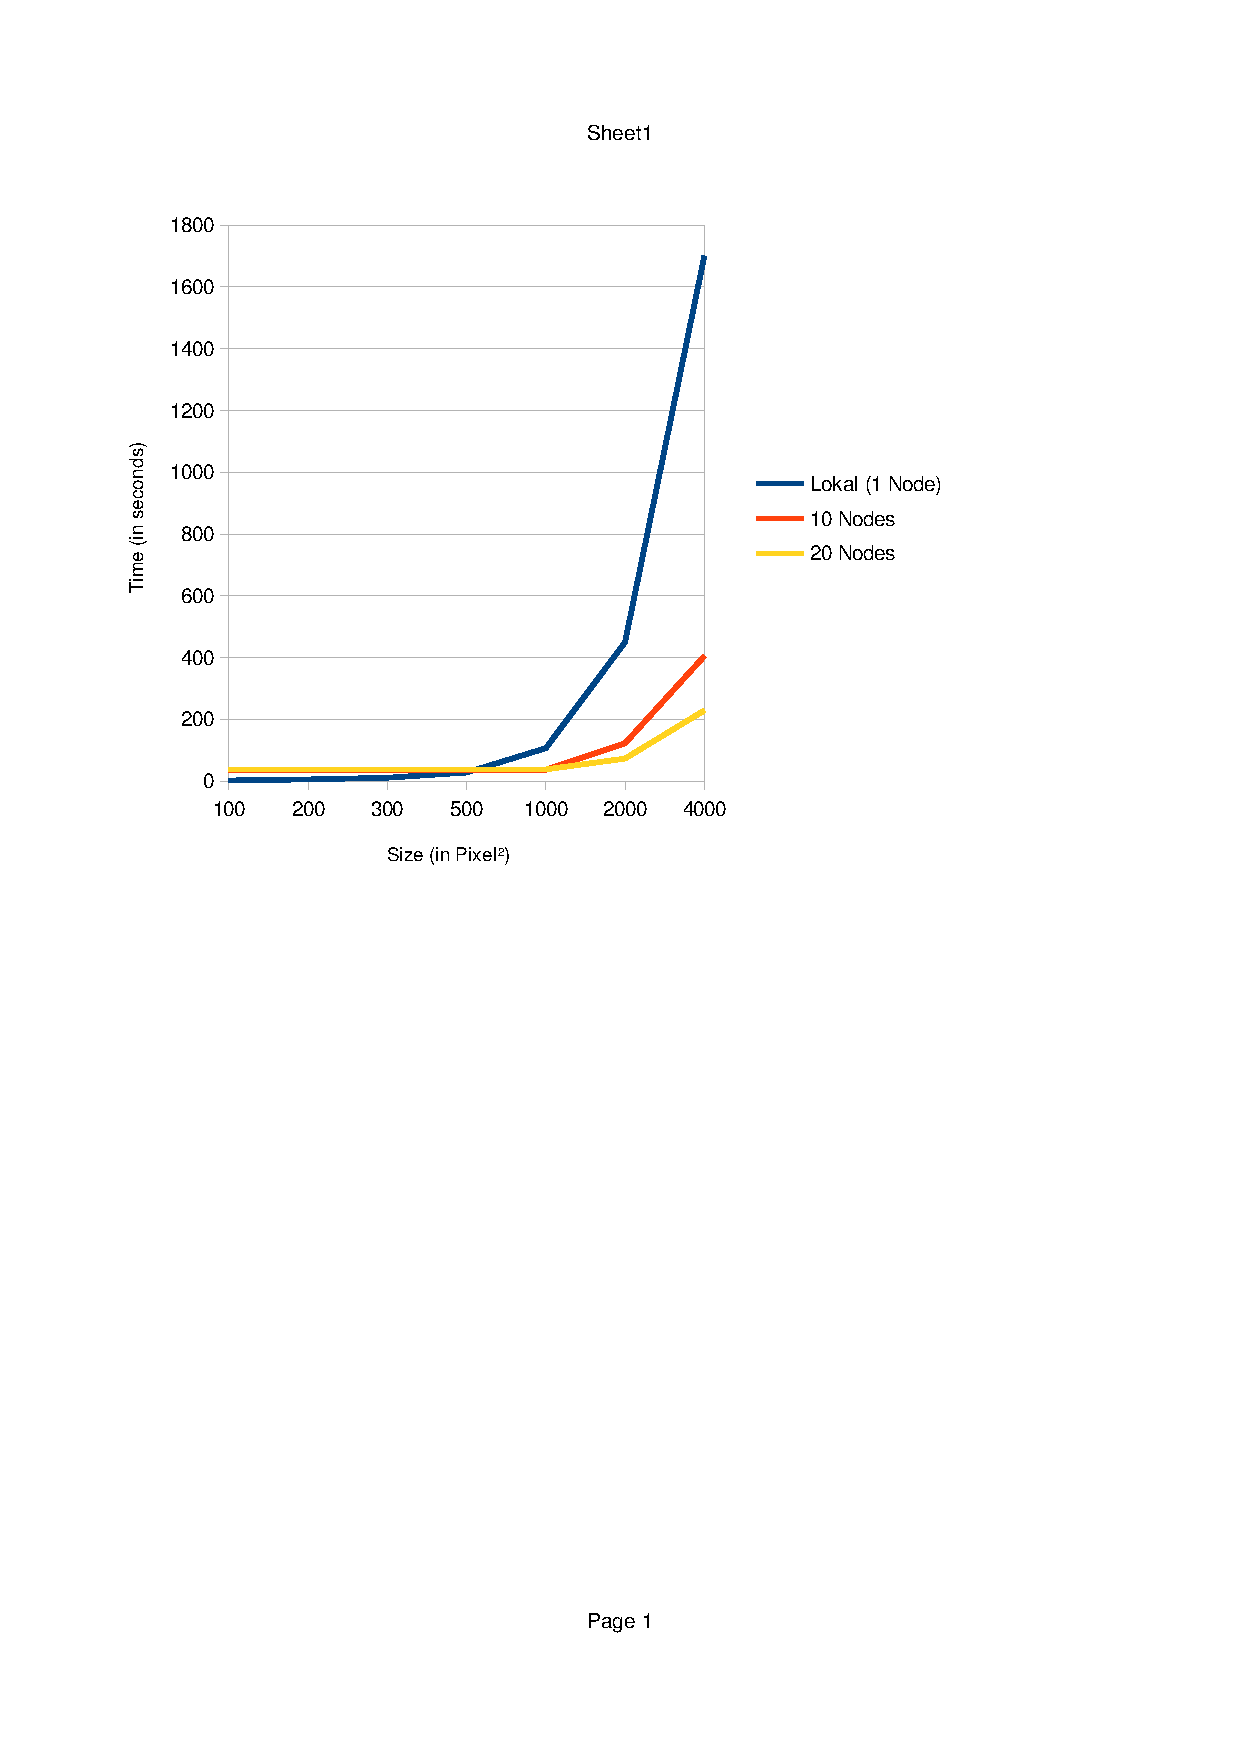
\includegraphics[trim=2cm 14cm 4cm 3cm,clip]{./task_03/plot}
			\end{center}
			\caption{Plot der Performanzauswertung.}
			\label{fig:povrayperfplot}
		\end{figure}
	

%\newpage
%\section{Aufgabenblatt 5}
\subsection{Cluster und Grid Computing}

	\subsubsection*{Zusammenhänge von Grid und Cluster Systemen}
	{\scriptsize Stichpunkte: \textsl{Virtual Organization, Grid Site, Cluster Management, Cluster Clients, Grid Server, Grid Clients, Information Service, Meta-Scheduler} } \\
	
		Grid Systeme sind lose Zusammenschlüsse von Computersystemen.
		Sie sind meist noch heterogener zusammengesetzt als Cluster Systeme.
		Grid werden von Virtuellen Organisationen verwendet.
		Sie gruppieren Gruppen von Benutzer nach definierten Eingenschaften
		und legen der Zugriffsrechte innerhalb des Grids fest.
		Die Verwaltung von Grid-Systemen erfolgt über eine Grid Middleware,
		welche der verbindende Punkt zwischen den einzelnen Grid Sites ist.
		
		Cluster können teile von Grids sein.
		Die Cluster werden dann zu Grid-Clients,
		welche durch den Meta-Scheduler des Grids Jobs zugewiesen bekommen.
		Die Jobs werden dann im Cluster auf die einzelnen Nodes verteilt.
		
		Das Grid-System wir durch den Information Service zusammengehalten.
		Es ermöglicht den Zugriff auf wichtige Daten des Gridsystems.
		Beispielsweise, welche Daten in welcher Gridsite lokal vorhanden sind,
		oder wie stark eine Ressource ausgelastet ist, bzw. verfügbar ist.

	\subsubsection*{Was ist ein Meta-Schedulder?}
		%ws-gram
	\subsubsection*{Vorteile von Grid gegenüber Clustersystemen}

\subsection{Zertifikate und Proxy}
	\subsubsection*{Wie werden Zertifikate verwendet?}
	\subsubsection*{Zusammenhang: Grid-Zertifikat, -Credentials, -Proxy, Credentials Delegation und öffentlicher Schlüssel}

	\subsubsection*{Prüfen von Grid-Zertifikaten}
	\subsubsection*{Prüfen von Grid-Proxy-Zertifikaten}
	\subsubsection*{Verändern von Grid-Proxy Zertifikaten}

\subsection{Grid-Umgebung}
	\subsubsection*{Service Container der Grid-Umgebung}
	\subsubsection*{Verfügbarkeit von Rssourcen in der Grid-Umgebeung}
	\subsubsection*{Datenverfügbarkeit in der Grid-Umgebung}
	% $> globus-url-copy && rft

\subsection{Job Submission mit dem Globus Toolkit}
	% $>globusrun-ws submit -f job.xml
	\subsubsection*{Unterschied zwischen Fork und PBS Job}
	\subsubsection*{Dokumentieren von Grid-Jobs}
		% MDS für Monitoring und Discovery
		% $>wsrf-query


%\newpage
\section{Aufgabenblatt 10}

\subsection{Assignment 1}
	\subsubsection{Blocking and non-blocking operations}
		The lecture slides define a blocking operation in the following way: 
		\textit{'Blocking: The return of the operation on a process ensures that the local resources (buffers) can be reused.'} 
		
		In contradiction, \textit{'a non-blocking operation does not guarantee that the local resources can be reused after returning to the process.}
		
		
	
	\subsubsection{Collective and point-to-point communication}
		

\end{document}
